\documentclass[portrait,final,a0paper,fontscale=0.277]{baposter}
\usepackage{float}
\usepackage{calc}
\usepackage{graphicx}
\usepackage{amsmath}
\usepackage{amssymb}
\usepackage{relsize}
\usepackage{multirow}
\usepackage{rotating}
\usepackage{bm}
\usepackage{url}
\usepackage{booktabs}
\usepackage[brazilian]{babel}
\usepackage[utf8x]{inputenc}

\usepackage{graphicx}
\usepackage{multicol}

%\usepackage[font-small, labelfont=bf]{caption}

%\usepackage{times}
%\usepackage{helvet}
%\usepackage{bookman}
\usepackage{palatino}

%\newcommand{\captionfont}{\footnotesize}

\graphicspath{{images/}{../images/}}
\usetikzlibrary{calc}

\newcommand{\SET}[1]  {\ensuremath{\mathcal{#1}}}
\newcommand{\MAT}[1]  {\ensuremath{\boldsymbol{#1}}}
\newcommand{\VEC}[1]  {\ensuremath{\boldsymbol{#1}}}
\newcommand{\Video}{\SET{V}}
\newcommand{\video}{\VEC{f}}
\newcommand{\track}{x}
\newcommand{\Track}{\SET T}
\newcommand{\LMs}{\SET L}
\newcommand{\lm}{l}
\newcommand{\PosE}{\SET P}
\newcommand{\posE}{\VEC p}
\newcommand{\negE}{\VEC n}
\newcommand{\NegE}{\SET N}
\newcommand{\Occluded}{\SET O}
\newcommand{\occluded}{o}

%%%%%%%%%%%%%%%%%%%%%%%%%%%%%%%%%%%%%%%%%%%%%%%%%%%%%%%%%%%%%%%%%%%%%%%%%%%%%%%%
%%%% Some math symbols used in the text
%%%%%%%%%%%%%%%%%%%%%%%%%%%%%%%%%%%%%%%%%%%%%%%%%%%%%%%%%%%%%%%%%%%%%%%%%%%%%%%%

%%%%%%%%%%%%%%%%%%%%%%%%%%%%%%%%%%%%%%%%%%%%%%%%%%%%%%%%%%%%%%%%%%%%%%%%%%%%%%%%
% Multicol Settings
%%%%%%%%%%%%%%%%%%%%%%%%%%%%%%%%%%%%%%%%%%%%%%%%%%%%%%%%%%%%%%%%%%%%%%%%%%%%%%%%
\setlength{\columnsep}{1.5em}
\setlength{\columnseprule}{0mm}

%%%%%%%%%%%%%%%%%%%%%%%%%%%%%%%%%%%%%%%%%%%%%%%%%%%%%%%%%%%%%%%%%%%%%%%%%%%%%%%%
% Save space in lists. Use this after the opening of the list
%%%%%%%%%%%%%%%%%%%%%%%%%%%%%%%%%%%%%%%%%%%%%%%%%%%%%%%%%%%%%%%%%%%%%%%%%%%%%%%%
\newcommand{\compresslist}{%
	\setlength{\itemsep}{1pt}%
	\setlength{\parskip}{0pt}%
	\setlength{\parsep}{0pt}%
}

%%%%%%%%%%%%%%%%%%%%%%%%%%%%%%%%%%%%%%%%%%%%%%%%%%%%%%%%%%%%%%%%%%%%%%%%%%%%%%
%%% Begin of Document
%%%%%%%%%%%%%%%%%%%%%%%%%%%%%%%%%%%%%%%%%%%%%%%%%%%%%%%%%%%%%%%%%%%%%%%%%%%%%%

\begin{document}
	
	%%%%%%%%%%%%%%%%%%%%%%%%%%%%%%%%%%%%%%%%%%%%%%%%%%%%%%%%%%%%%%%%%%%%%%%%%%%%%%
	%%% Here starts the poster
	%%%---------------------------------------------------------------------------
	%%% Format it to your taste with the options
	%%%%%%%%%%%%%%%%%%%%%%%%%%%%%%%%%%%%%%%%%%%%%%%%%%%%%%%%%%%%%%%%%%%%%%%%%%%%%%
	% Define some colors
	
	%\definecolor{lightblue}{cmyk}{0.83,0.24,0,0.12}
	\definecolor{lightblue}{cmyk}{0,0.47,0.82,0.62}
	%\definecolor{lightblue}{rgb}{0.145,0.6666,1}
	%definecolor{lightblue}{rgb}{0.255,0.51,0.51}
	
	% Draw a video
	\newlength{\FSZ}
	\newcommand{\drawvideo}[3]{% [0 0.25 0.5 0.75 1 1.25 1.5]
		\noindent\pgfmathsetlength{\FSZ}{\linewidth/#2}
		\begin{tikzpicture}[outer sep=0pt,inner sep=0pt,x=\FSZ,y=\FSZ]
		\draw[color=lightblue!50!black] (0,0) node[outer sep=0pt,inner sep=0pt,text width=\linewidth,minimum height=0] (video) {\noindent#3};
		\path [fill=lightblue!50!black,line width=0pt] 
		(video.north west) rectangle ([yshift=\FSZ] video.north east) 
		\foreach \x in {1,2,...,#2} {
			{[rounded corners=0.6] ($(video.north west)+(-0.7,0.8)+(\x,0)$) rectangle +(0.4,-0.6)}
		}
		;
		\path [fill=lightblue!50!black,line width=0pt] 
		([yshift=-1\FSZ] video.south west) rectangle (video.south east) 
		\foreach \x in {1,2,...,#2} {
			{[rounded corners=0.6] ($(video.south west)+(-0.7,-0.2)+(\x,0)$) rectangle +(0.4,-0.6)}
		}
		;
		\foreach \x in {1,...,#1} {
			\draw[color=lightblue!50!black] ([xshift=\x\linewidth/#1] video.north west) -- ([xshift=\x\linewidth/#1] video.south west);
		}
		\foreach \x in {0,#1} {
			\draw[color=lightblue!50!black] ([xshift=\x\linewidth/#1,yshift=1\FSZ] video.north west) -- ([xshift=\x\linewidth/#1,yshift=-1\FSZ] video.south west);
		}
		\end{tikzpicture}
	}
	
	\hyphenation{resolution occlusions}
	%%
	\begin{poster}%
		% Poster Options
		{
			% Show grid to help with alignment
			grid=false,
			% Column spacing
			colspacing=1em,
			% Color style
			bgColorOne=white,
			bgColorTwo=white,
			borderColor=lightblue,
			headerColorOne=black,
			headerColorTwo=lightblue,
			headerFontColor=white,
			boxColorOne=white,
			boxColorTwo=lightblue,
			% Format of textbox
			textborder=roundedleft,
			% Format of text header
			eyecatcher=true,
			headerborder=closed,
			headerheight=0.1\textheight,
			%  textfont=\sc, An example of changing the text font
			headershape=roundedright,
			headershade=shadelr,
			headerfont=\Large\bf\textsc, %Sans Serif
			textfont={\setlength{\parindent}{1.5em}},
			boxshade=plain,
			%  background=shade-tb,
			background=plain,
			linewidth=2pt
		}
		% Eye Catcher
		{
\includegraphics[height=6.25em]{University_of_Tsukuba_logo.png}} 
		% Title
		{\bf\textsc{Experimental Analysis of the Tournament Size on Genetic Algorithms}\normalsize}
		% Authors
		{ \normalsize Yuri Cossich Lavinas$^1$ Claus Aranha$^1$  Marcelo Ladeira$^2$\\ $^1$Tsukuba University, Graduate School of Systems and Information Engineering, Japan\\ $^2$University of Brasilia, Computer Science Department}
		% University logo
		%{% The makebox allows the title to flow into the logo, this is a hack because of the L shaped logo.
		%\includegraphics[width=25.0em]{logo2.jpg}}
		
		%}
		
		%%%%%%%%%%%%%%%%%%%%%%%%%%%%%%%%%%%%%%%%%%%%%%%%%%%%%%%%%%%%%%%%%%%%%%%%%%%%%%
		%%% Now define the boxes that make up the poster
		%%%---------------------------------------------------------------------------
		%%% Each box has a name and can be placed absolutely or relatively.
		%%% The only inconvenience is that you can only specify a relative position 
		%%% towards an already declared box. So if you have a box attached to the 
		%%% bottom, one to the top and a third one which should be in between, you 
		%%% have to specify the top and bottom boxes before you specify the middle 
		%%% box.
		%%%%%%%%%%%%%%%%%%%%%%%%%%%%%%%%%%%%%%%%%%%%%%%%%%%%%%%%%%%%%%%%%%%%%%%%%%%%%%
		%
		% A coloured circle useful as a bullet with an adjustably strong filling
		\newcommand{\colouredcircle}{%
			\tikz{\useasboundingbox (-0.2em,-0.32em) rectangle(0.2em,0.32em); \draw[draw=black,fill=lightblue,line width=0.03em] (0,0) circle(0.18em);}}
		
		%%%%%%%%%%%%%%%%%%%%%%%%%%%%%%%%%%%%%%%%%%%%%%%%%%%%%%%%%%%%%%%%%%%%%%%%%%%%%%
		\headerbox{Introduction}{name=problem,column=0,row=0}{
			%%%%%%%%%%%%%%%%%%%%%%%%%%%%%%%%%%%%%%%%%%%%%%%%%%%%%%%%%%%%%%%%%%%%%%%%%%%%%%
			\vspace{-0.3em}
			Genetic Algorithm (GA) is composed of: 
			
			\begin{itemize}
				\item crossover operator (new solutions)\vspace{-1em}
				\item mutation operator (sustain diversity)\vspace{-1em}
				\item selection operator (select solutions to compose new population)
			\end{itemize} 
			
			One of the most used selection is the tournament operator which has one parameter, the tournament size (K).
			
			This parameter is said to adjust the balance between the exploration and explotation.
			
			Goal: Observe the performance of the tournament selection in a real-valued Genetic Algorithm to learn the role of K.
			
		}\vspace{-1em}
		
		%%%%%%%%%%%%%%%%%%%%%%%%%%%%%%%%%%%%%%%%%%%%%%%%%%%%%%%%%%%%%%%%%%%%%%%%%%%%%%
		\vspace{-1em}
		\headerbox{Tournament Selection}{name=model,column=0,below=problem}{
			%%%%%%%%%%%%%%%%%%%%%%%%%%%%%%%%%%%%%%%%%%%%%%%%%%%%%%%%%%%%%%%%%%%%%%%%%%%%%%
			\begin{itemize}
				\item K candidates are sampled randomly and the one with best fitness is selected\vspace{-1em}
				\item Controlling the tournament size - expect to adjust the balance exploration X explotation\vspace{-1em}
				\item The selection pressure is expected to increase with larger tournament size values\vspace{-1em}
				\item Review of the literature shows a preference to small values for the tournament size, such as as 2 or 3\vspace{-1em}
				\item Little experimental justification% \vspace{-1em}
			\end{itemize}
			
		}%\vspace{-1em}
		
		%%%%%%%%%%%%%%%%%%%%%%%%%%%%%%%%%%%%%%%%%%%%%%%%%%%%%%%%%%%%%%%%%%%%%%%%%%%%%%
		\headerbox{Experiment Design}{name=metodologia,column=0,below=model}{\vspace{-0.3em}
			\begin{itemize}
				\item Real-valued GA, with solution's value between [-4,4]\vspace{-1em}
				\item Configuration: Uniform crossover (0.9), elitism (1), Gaussian mutation (0.1, mean=0, std=0, prob, attribute to mutate-0.1) \vspace{-1em}
				\item Fitness Functions: 24 noise-free BBOB benchmark functions with 10, 20 and 40 dimensions\vspace{-1em}
				\item Tournament sizes: 2 to 25
			\end{itemize} 
		}
		\vspace{3em}
		\headerbox{Statistical Analysis}{name=boxplot2009,column=0,above=bottom}{
			%%%%%%%%%%%%%%%%%%%%%%%%%%%%%%%%%%%%%%%%%%%%%%%%%%%%%%%%%%%%%%%%%%%%%%%%%%%%%%
			\centering
			\begin{center}
				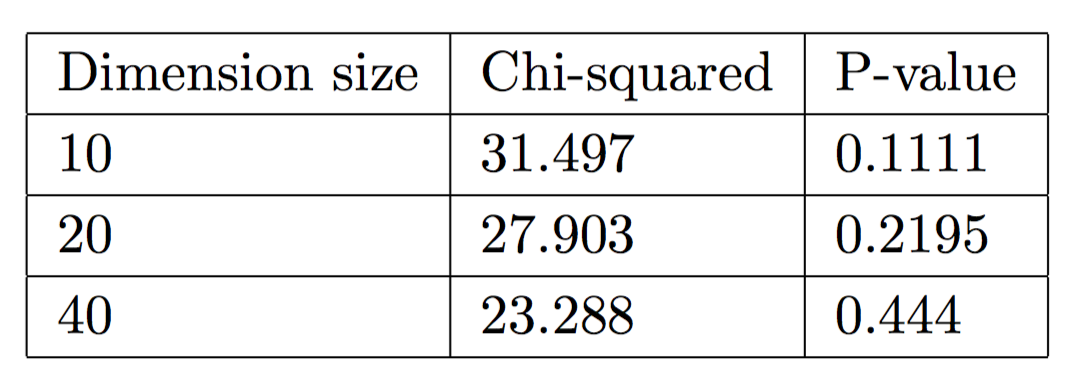
\includegraphics[width=1.\textwidth]{images/friedmantest.png}\\
				\normalsize{Friedman Test on the effect of K given all functions}
			\end{center} 
			
			\vspace{-1em}
		}   
		
		%%%%%%%%%%%%%%%%%%%%%%%%%%%%%%%%%%%%%%%%%%%%%%%%%%%%%%%%%%%%%%%%%%%%%%%%%%%%%%
		\headerbox{Observed Impact of the Tournament Size by Functions}{name=results,column=1,span=2,row=0}{
			
			%%%%%%%%%%%%%%%%%%%%%%%%%%%%%%%%%%%%%%%%%%%%%%%%%%%%%%%%%%%%%%%%%%%%%%%%%%%%%%
			The Figures below show that \textbf{changing the tournament size} does not lead to significant better final values found by the GA. The gray shaded area represents the 95\% confidence level interval (predictions from a linear model) for each scenario. For all Figures, the mean of 40 repetitions is shown as bullets and the bars represent the standard deviation. All Figures show from left to right the results for 10, 20, 40 Dimensions. The red lines in the bottom of the Figures show the target value for each function.
			\begin{center}
				
				\large{Performance on different tournament size for the Linear Slope Function.}\\
				\raggedleft
				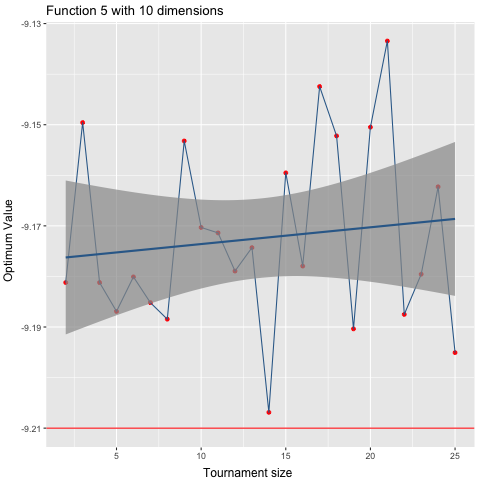
\includegraphics[width=0.32\textwidth]{5dim_10.png}
				\centering
				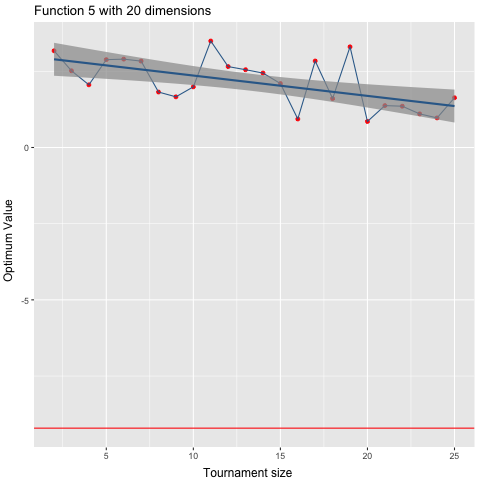
\includegraphics[width=0.32\textwidth]{5dim_20.png}
				\raggedright
				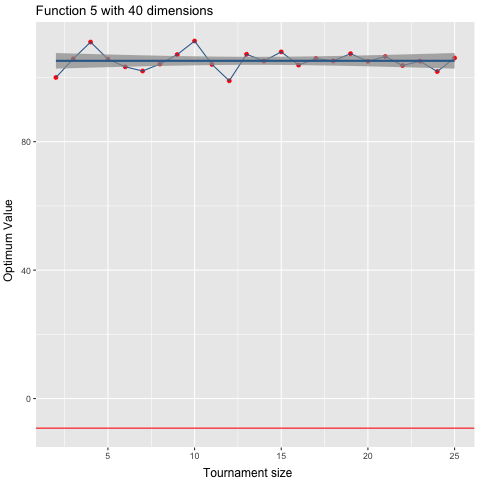
\includegraphics[width=0.32\textwidth]{5dim_40.png}
				
				\large{Performance on different tournament size for the Bent Cigar Function.}\\
				\raggedleft
				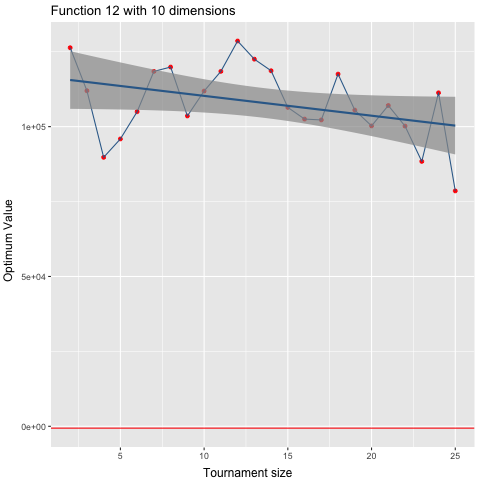
\includegraphics[width=0.32\textwidth]{12dim_10.png}
				\centering
				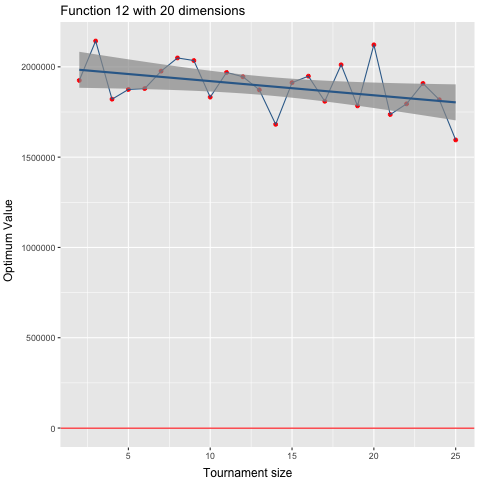
\includegraphics[width=0.32\textwidth]{12dim_20.png}
				\raggedright
				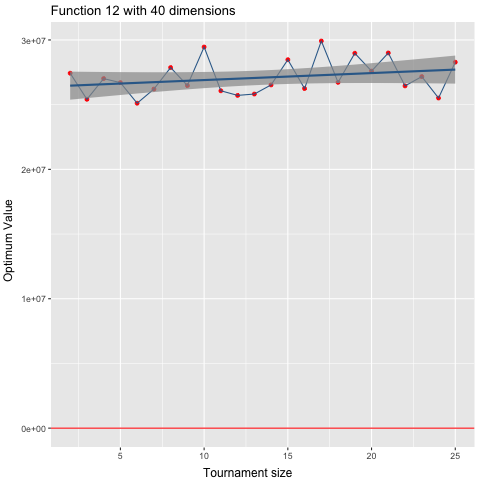
\includegraphics[width=0.32\textwidth]{12dim_40.png}
				
				\large{Performance on different tournament size for the Gallagher’s Gaussian 101-me Peaks Function.}\\
				\raggedleft
				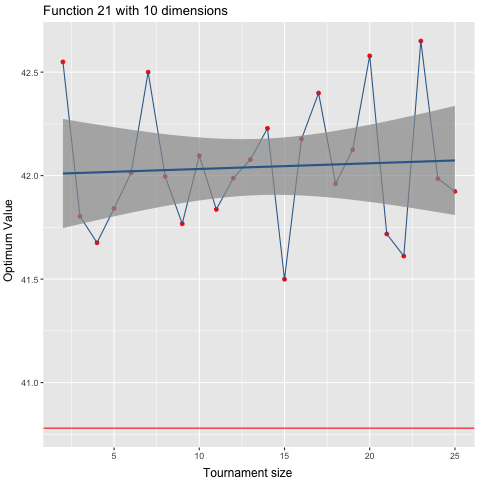
\includegraphics[width=0.32\textwidth]{21dim_10.png}
				\centering
				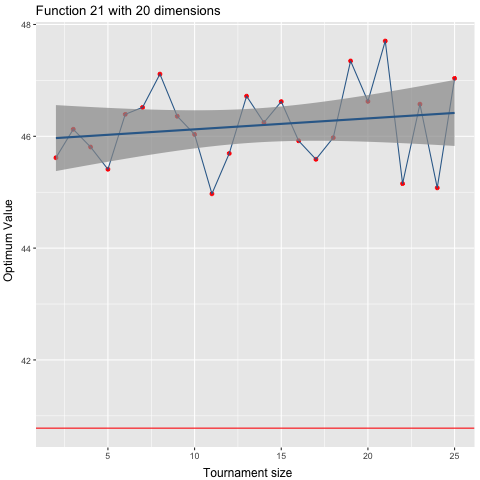
\includegraphics[width=0.32\textwidth]{21dim_20.png}
				\raggedright
				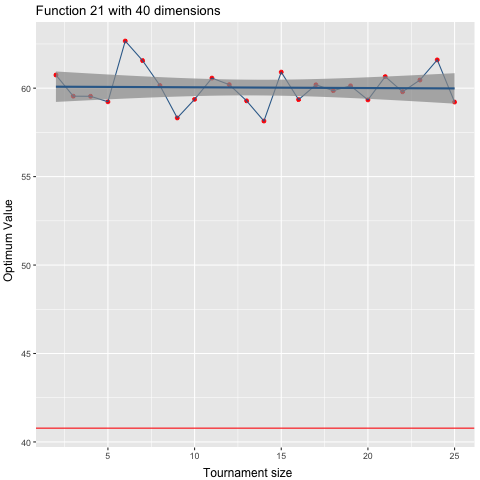
\includegraphics[width=0.32\textwidth]{21dim_40.png}
				
				
				
			\end{center}
			
			
			%%%%%%%%%%%%%%%%%%%%%%%%%%%%%%%%%%%%%%%%%%%%%%%%%%%%%%%%%%%%%%%%%%%%%%%%%%%%%
			\vspace{-1.em}
		}
		
		\headerbox{Preliminary self-adaptative tournament size}{name=bigGraph,column=1,span=2,row=0, below=results}{
			%%%%%%%%%%%%%%%%%%%%%%%%%%%%%%%%%%%%%%%%%%%%%%%%%%%%%%%%%%%%%%%%%%%%%%%%%%%%%%
			The Figures below preliminary results of the self-adaptative tournament size when \textbf{half of the evaluations are completed}. The gray shaded area represents the 95\% confidence level interval for predictions from a linear model for each scenario showed and demonstrate that no value of the tournament size has consistently better results. For all Figures, the mean of 40 repetitions is shown as bullets and the bars represent the standard deviation. The red lines in the bottom of the Figures show the target value for each function.
			\begin{center}
				\large{Performance for the Linear Slope Function,Bent Cigar Function with 40-D.}\\
				\raggedleft
				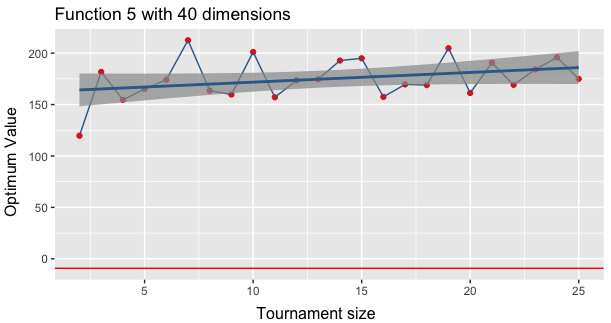
\includegraphics[width=0.48\textwidth]{5dim_40_pseudo.png}
				\centering
				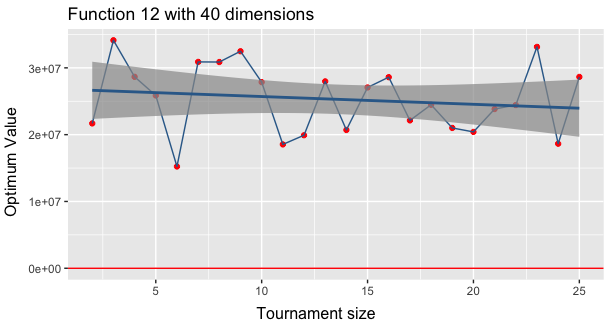
\includegraphics[width=0.48
				\textwidth]{12dim_40_pseudo.png}
				% \raggedright
				% 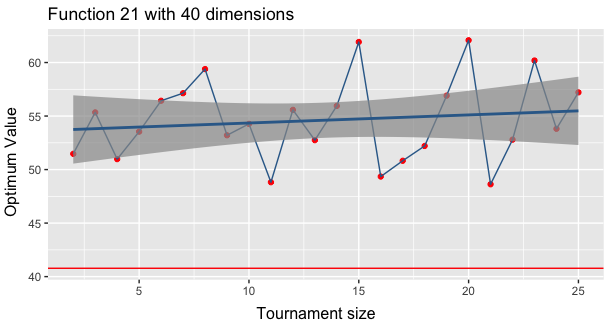
\includegraphics[width=0.32\textwidth]{21dim_40_pseudo.png}
			\end{center}
			\vspace{-1.em}
		}
		
		%%%%%%%%%%%%%%%%%%%%%%%%%%%%%%%%%%%%%%%%%%%%%%%%%%%%%%%%%%%%%%%%%%%%%%%%%%%%%%
		\headerbox{Discussion}{name=references,column=0, below=metodologia}{
			%%%%%%%%%%%%%%%%%%%%%%%%%%%%%%%%%%%%%%%%%%%%%%%%%%%%%%%%%%%%%%%%%%%%%%%%%%%%%%
			%\centering
			\begin{itemize}
				\item We found no significant relationship between the tournament size values and the final quality\vspace{-1.em}
				\item A better understanding of the role of the tournament size in the final quality is necessary\vspace{-1.em}
				\item We want to explore this effect on other GA operators, including self-adaptative approaches
			\end{itemize}
			\vspace{-1.em}
		}
	\end{poster}
	
\end{document}

